\documentclass[handout]{beamer}

\usepackage{algorithm,algorithmic}
\usepackage{biblatex}
\usepackage{amsmath,mathtools}
\usepackage{physics}
\graphicspath{{../assets/}}
\addbibresource{bibliography.bib}

\parskip=10pt

\newcommand{\myvec}[1]{\ensuremath{\begin{pmatrix}#1\end{pmatrix}}}

\usetheme{CambridgeUS}

\title{Complex Networks}
\author{Shoichi Yip}
\institute{M2 PCS}
\date{3 April 2024}

\begin{document}

\frame{\titlepage}

\section{Random graphs of the configuration model}

\begin{frame}{Complex networks}
    \alert{Networks} are often the backbone of many complex systems.

    Biological systems, citations in papers, social networks can be all modeled
    as complex networks.

    The modeling of complex networks has stem from the study of
    \alert{models of random graphs}, starting with the pioneering work by Paul
    Erd\H{o}s and Alfr\'{e}d R\'{e}nyi in 1959.
\end{frame}

\begin{frame}{Random graphs}
\end{frame}

\begin{frame}{The problem with ER graphs}
    Graphs generated using the ER model have a Poisson degree distribution.

    However, experimental study of real world graphs show us that most of the
    times they do not follow a Poissonian behaviour.

    We can overcome this problem by using the \alert{configuration model}.
\end{frame}

\begin{frame}{The configuration model}
    The \alert{configuration model} allows us to generate graphs exactly with a
    given \alert{degree sequence} $\vec k$.

    The degree sequence is a vector, for example,
    $$
    \vec k = \myvec{3 & 2 & 3 & 1 & 1}
    $$
    where each $i$-th element is the degree of the $i$-th node.
\end{frame}

\begin{frame}{Sampling a graph from a configuration model}
    The configuration model provides us with a constructive algorithm in order
    to find an instance of a random graph, provided a degree sequence $\vec k$.

    For example, if we take the $\vec k$ degree sequence from the previous slide
    we can start with a set of unconnected nodes where each $i$-th node has
    $k_i$ \alert{stubs}, or half-edges.

    Then we get a random graph instance by taking two random stubs at a time and
    connecting them. On general grounds, the configuration model allows for the
    presence of multiple edges and self-edges.
\end{frame}

\begin{frame}{Sampling a graph from a configuration model}
    \begin{figure}
        \centering
        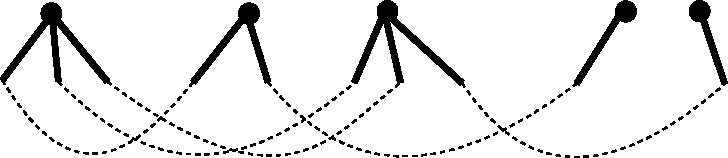
\includegraphics[width=.4\textwidth]{config_model}
        \caption{Connecting stubs in the configuration model}
        \label{fig:config_model}
    \end{figure}
\end{frame}

\begin{frame}{Configuration model given a degree distribution}
    We can adapt the configuration model to a specific task, that of sampling
    graphs that have a specific \alert{degree distribution}.

    We can in fact first of all define a degree sequence such that the abundance
    of nodes of degree $d$ are given by a degree distribution $p_d$. Then we can
    proceed as we would do for the configuration model, by wiring the stubs.

    We can hence extract random graph instances that nearly exactly match the
    degree distribution.
\end{frame}

\begin{frame}{Our ensemble}
    In our particular case, we define a random graph ensemble $\mathcal{G}$ such
    that:
    \begin{itemize}
        \item the graph has $N$ nodes;
        \item the graph is generated using the configuration model;
        \item the graph \alert{does not} contain self-edges and multiple edges;
        \item we define a parameter $\pi$ and the the graph is such that the
            fraction of the nodes $p_1 = 1-\pi$ has degree 1, and the remaining
            fraction $p_4 = \pi$ has degree 4.
    \end{itemize}
\end{frame}

\begin{frame}{Algorithm to generate RG instance}
    \begin{algorithm}[H]
        \begin{algorithmic}[1]
            \FOR{$k_i$ in degree sequence $\vec k$}
                \STATE Generate node with $k_i$ stubs
            \ENDFOR
            \WHILE{Graph $G$ not generated}
                \WHILE{Stub list is not exhausted}
                    \STATE Pick two random stubs
                    \STATE Create a candidate edge between them
                    \STATE Check whether they are not multiedge or self-edge
                \ENDWHILE
            \ENDWHILE
        \end{algorithmic}
        \caption{Algorithm to generate stubs and connect them}
    \end{algorithm}
\end{frame}

\begin{frame}{Examples of random graphs}
    \begin{figure}
        \centering
        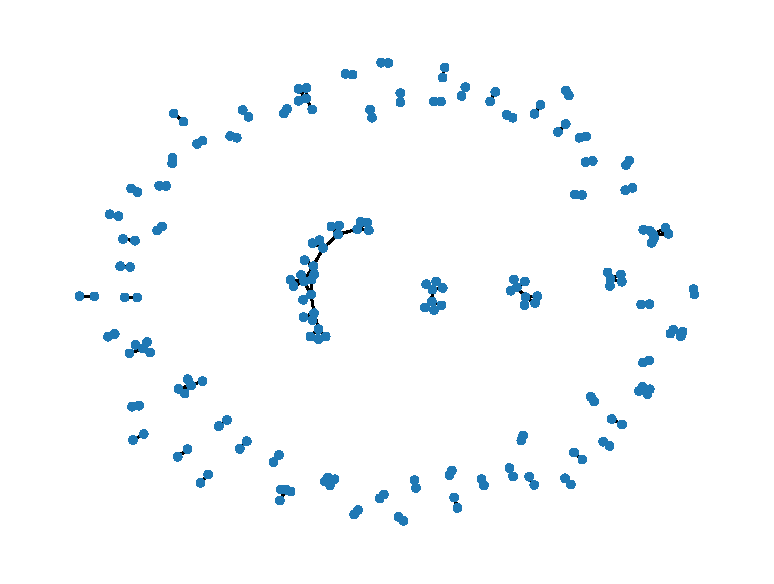
\includegraphics[height=.7\textheight]{rg0}
        \caption{Instance of a random graph for $\pi=0.1$}
        \label{fig:rg0}
    \end{figure}
\end{frame}

\begin{frame}{Examples of random graphs}
    \begin{figure}
        \centering
        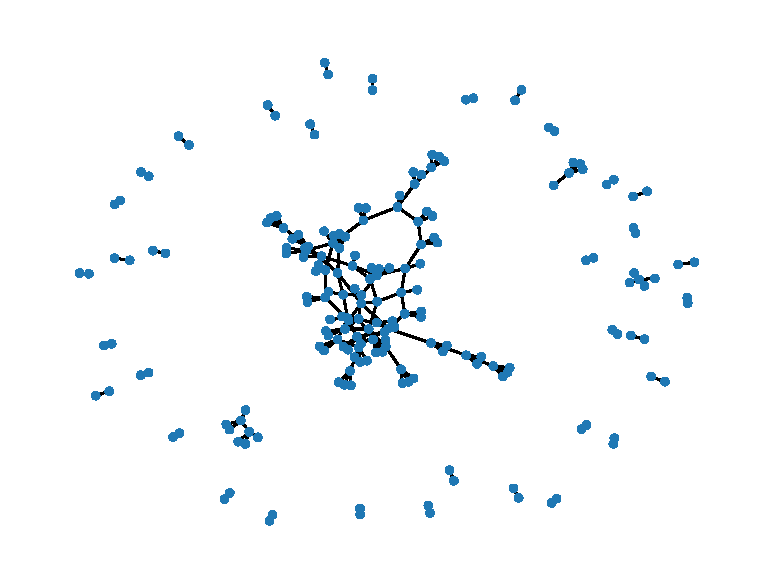
\includegraphics[height=.7\textheight]{rg1}
        \caption{Instance of a random graph for $\pi=0.3$}
        \label{fig:rg1}
    \end{figure}
\end{frame}

\begin{frame}{Examples of random graphs}
    \begin{figure}
        \centering
        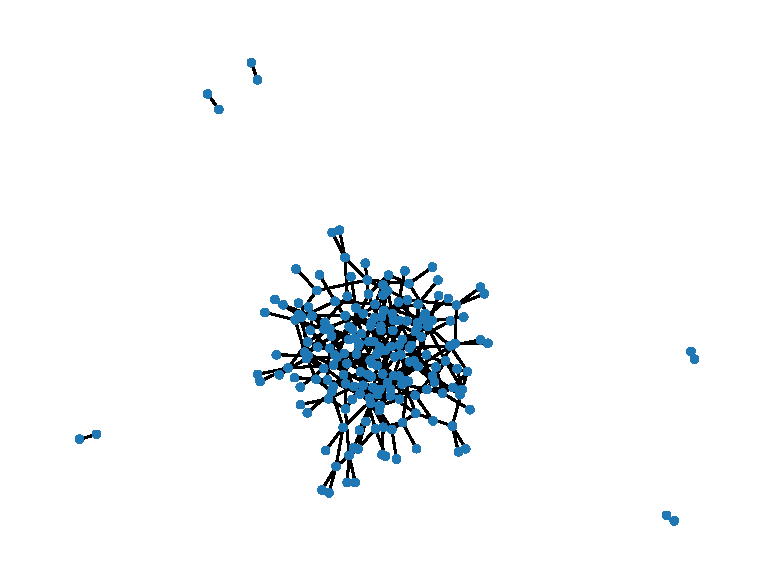
\includegraphics[height=.7\textheight]{rg2}
        \caption{Instance of a random graph for $\pi=0.7$}
        \label{fig:rg2}
    \end{figure}
\end{frame}

\section{The giant component}

\begin{frame}{The giant component}
\end{frame}

\begin{frame}{Detecting the giant component in an instance}
\end{frame}

\begin{frame}{The onset of criticality}
\end{frame}

\begin{frame}{Size of the giant component}
    In order to find the size of the giant component we resort to the study of
    the probability that an excess node or a node belongs to the giant
    component \cite[56]{weigt}.

    \begin{figure}
        \centering
        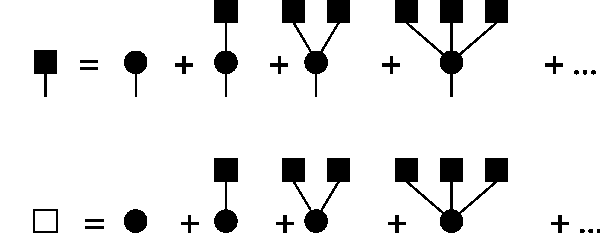
\includegraphics[width=.6\textwidth]{PTCOP_iterative}
        \caption{Scheme for the iterative solution to find the probability that
        a node belongs to the giant component and the excess probability}
        \label{fig:iterative}
    \end{figure}
\end{frame}

\begin{frame}{Excess probability that node belongs to GC}
    The scheme reads as follows. The excess proability $\mu$, which is
    the probability that given a randomly selected edge one of its end vertices
    is not connected with a GC, is given by
    \begin{itemize}
        \item the probability that the excesss node has degree 1, i.e. there
            would not exist any other edge that connects it to a GC
        \item the probability that the excess node is connected to a node that
            does not belong to the GC
        \item the probability that the excess node is connected to two nodes
            that do not belong to the GC
        \item etc.
    \end{itemize}
\end{frame}

\begin{frame}{Probability that node belongs to GC}
    The same goes for the probability that a randomly selected node does not
    belong to the GC. The proability $1-\gamma$, is given by
    \begin{itemize}
        \item the probability that this node is isolated
        \item the probability that this node is connected to a node that does
            not belong to the GC
        \item the probability that this node is connected to two nodes that do
            not belong to the GC
        \item etc.
    \end{itemize}
\end{frame}

\begin{frame}{Iterative equations}
    We then find the iterative equations, respectively
    \begin{equation}
        \begin{cases}
            \mu = q_1 + q_2 \mu + q_3 \mu^2 + ...\\
            1 - \gamma = p_0 + p_1 \mu + p_2 \mu^2 + ...
        \end{cases}
        \label{eq:iterative}
    \end{equation}

    Since our degree distribution has only two nonzero terms for $d=1$ and
    $d=4$, sd can rewrite them as
    \begin{equation}
        \begin{cases}
            \mu = q_1 + q_4 \mu^3\\
            1 - \gamma = p_1 \mu + p_4 \mu^4
        \end{cases}
        \label{eq:iterative_cm}
    \end{equation}
\end{frame}

\begin{frame}{}
    We can solve the first third order equation in Eq.~\ref{eq:iterative_cm} and
    we get
    $$
    \mu = 1 \quad \lor \quad \mu = \frac{-1-\sqrt{\pi}}{2\sqrt{\pi}} \quad
    \lor \quad \mu = \frac{1-\sqrt{\pi}}{2\sqrt{\pi}}
    $$
    where the first solution is the trivial solution that does not have any
    giant component, and the second solution is negative (so it cannot be a
    probability). If we plug the third solution in the second equation we get
    \begin{equation}
        \gamma = 1 - (1-\pi) \frac{1-\sqrt{\pi}}{2\sqrt{\pi}} - \pi \left(
        \frac{1-\sqrt{\pi}}{2\sqrt{\pi}} \right)^4
        \label{eq:gamma_final}
    \end{equation}
    which gives us the theoretical value of the probability of a node being part
    of the GC, hence also the expectation value over the size of the GC.
\end{frame}

\begin{frame}{The size of the giant component}
    \begin{figure}
        \centering
        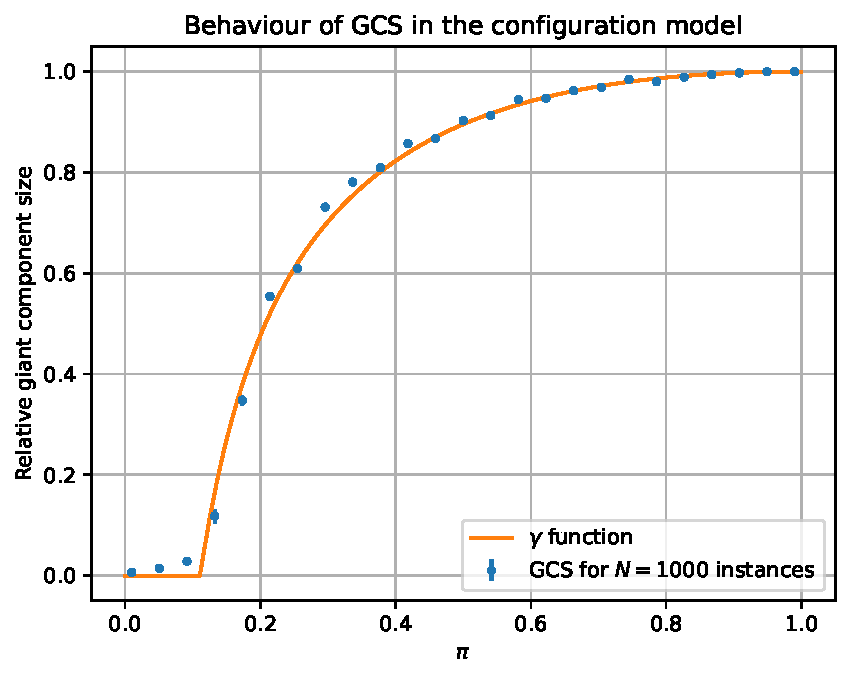
\includegraphics[height=.7\textheight]{gcs}
        \caption{Comparison between theoretical value and measures from random
        instances of the size of the giant component}
        \label{fig:gcs}
    \end{figure}
\end{frame}

\section{Emergence of $q$-cores}

\begin{frame}{The deterministic $q$-core algorithm}
    The $q$-core of a graph can be found using a simple algorithm.

    \begin{algorithm}[H]
        \begin{algorithmic}[1]
            \WHILE{Nodes with $d < q$ are present}
                \STATE Remove all nodes with $d<q$
            \ENDWHILE
        \end{algorithmic}
        \caption{Algorithm for deterministic $q$-core detection}
        \label{algo:qcore_det}
    \end{algorithm}

    We will use this algorithm to find the size of a $q$-core.
\end{frame}

\begin{frame}{The stochastic $q$-core algorithm}
    There is a stochastic version of this algorithm.

    \begin{algorithm}[H]
        \begin{algorithmic}[1]
            \WHILE{Nodes with $d < q$ are present}
            \STATE{Select randomly a node with degree $d < q$}
            \IF{The node has degree $d < q$}
            \STATE{Remove node}
            \ENDIF
            \ENDWHILE
        \end{algorithmic}
        \caption{Algorithm for stochastic $q$-core detection}
        \label{algo:qcore_stoc}
    \end{algorithm}

    This algorithm does not remove an extensive amount of nodes for each
    timestep and its dynamic can be described by an ODE.
\end{frame}

\begin{frame}{Rate equations for the $q$-core}
    The behaviour of $q$-cores in Algorithm~\ref{algo:qcore_stoc} can be
    described by \alert{rate equations} using the \alert{Wormwald method}.
    \cite[58]{weigt}.

    The algorithmic time $N(T) = N - T$ describes the amount of nodes that are
    still available, where $N$ is the total number of nodes and $T$ is the
    number of nodes that we have removed.

    We can introduce a \alert{rescaled time} $t = T / N$, which will span from 0
    to 1.

    The variable that we want to study in time is the \alert{degree
    distribution at time $t$}
    \begin{equation}
        p_d(t) = \frac{N_d(t)}{N(t)} = \frac{N_d(t)}{N[1-t]}
        \label{eq:deg_time}
    \end{equation}
\end{frame}

\begin{frame}{ODE for the rate equation}
    We can write the difference between two consecutive timesteps of the number
    of nodes of degree $d$ as
    \begin{equation}
        N_d(T+1) - N_d(T) =
        - \frac{\chi_d p_d}{\overline \chi_d}
        + \frac{\overline{\chi_d d}}{\overline \chi_d c(t)}
        [(d+1) p_{d+1}(t) - dp_d(t)]
        \label{eq:diff_ndeg}
    \end{equation}
    where $\chi_d$ is the \alert{indicator function}
    \begin{equation}
        \chi_d =
        \begin{cases*}
            1 & if $d<q$\\
            0 & if $d\geq q$
        \end{cases*}
        \label{eq:indfunc}
    \end{equation}
    and $c(t)$ is the average connectivity at time $t$
    \begin{equation}
        c(t) = \sum_d d p_d(t)
        \label{eq:avgcon}
    \end{equation}
\end{frame}

\begin{frame}{ODE for the rate equation}
    Starting from Eq.~\ref{eq:diff_ndeg} we can find the equations for $p_d(t)$
    \begin{equation}
        \partial_t[(1-t) p_d(t)] = - \frac{\chi_d p_d}{\overline \chi_d}
        + \frac{\overline{d \chi_d}}{c(t) \overline \chi_d}
        [(d+1) p_{d+1}(t) - d p_d(t)]
        \label{eq:wormwald_ode}
    \end{equation}
    
    Since we \alert{start} with finite $p_d(0)$ for $d=1,4$, we will have
    nonzero terms for $t>0$ for $d=0,1,2,3,4$. In fact, by randomly removing a
    node and its attached edges, we might decrease the degrees of its previously
    attached nodes.
\end{frame}

\begin{frame}{ODE for the rate equation}
    For our specific problem, if we define
    $$
    A(t) = \frac{1}{p_0(t) + p_1(t) + p_2(t)}
    \quad B(t) = \frac{p_1(t) + 2 p_2(t)}{c(t)} A(t)
    $$
    we get the system of equations
    {\scriptsize
    \begin{align*}
        \dv{p_0(t)}{t} &= \frac{1-A(t)}{1-t} p_0(t) + \frac{B(t)}{1-t} p_1(t)\\
        \dv{p_1(t)}{t} &= \frac{1-A(t)-B(t)}{1-t} p_1(t) + \frac{2B(t)}{1-t} p_2(t)\\
        \dv{p_2(t)}{t} &= \frac{1-A(t)-2B(t)}{1-t} p_2(t) + \frac{3B(t)}{1-t}
        p_3(t)\\
        \dv{p_3(t)}{t} &= \frac{1-3B(t)}{1-t} p_3(t) + \frac{4B(t)}{1-t} p_4(t)\\
        \dv{p_4(t)}{t} &= \frac{1-4B(t)}{1-t} p_4(t)
    \end{align*}
    where
    $$
    p_0(0) = 0 \quad p_1(0) = 1-\pi \quad p_2(0)=0 \quad p_3(0)=0 \quad
    p_4(0)=\pi
    $$
    }
\end{frame}

\begin{frame}{ODE for the rate equation}
    We can rephrase the ODE as
    \begin{equation}
        \dv{\vec p(t)}{t} = M(t) \vec p(t)
    \end{equation}
    where
    {\scriptsize
    $$
    M(t) = \frac{1}{1-t}
    \begin{pmatrix}
        1-A(t) & B(t) & 0 & 0 & 0\\
        0 & 1-A(t)-B(t) & 2B(t) & 0 & 0\\
        0 & 0 & 1-A(t)-2B(t) & 2B(t) & 0\\
        0 & 0 & 0 & 1-3B(t) & 4B(t)\\
        0 & 0 & 0 & 0 & 1-4B(t)
    \end{pmatrix}
    $$
    }
\end{frame}

\begin{frame}{The size of the 3-core}
    \begin{figure}
        \centering
        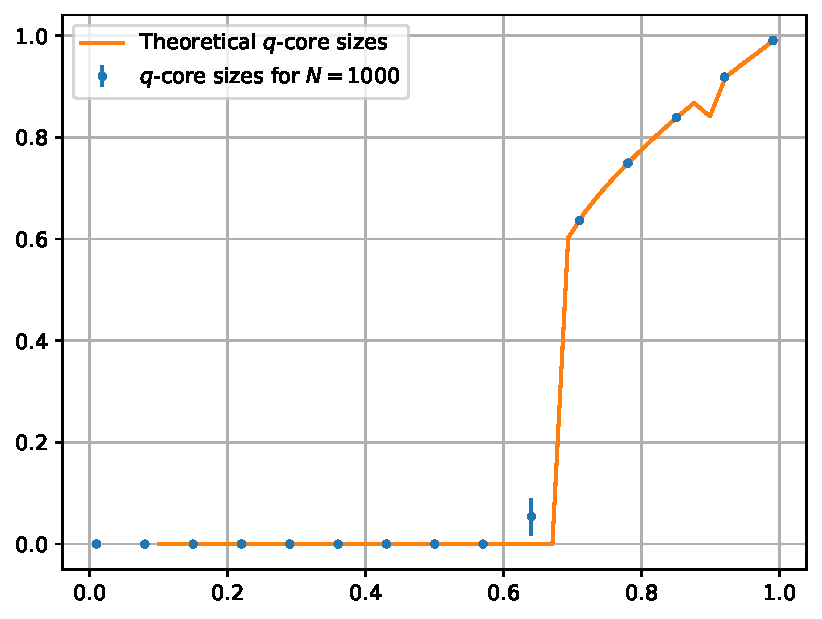
\includegraphics[height=.7\textheight]{qcore}
        \caption{Comparison between theoretical value and measures from random
        instances of the size of the 3-core}
        \label{fig:qcore}
    \end{figure}
\end{frame}

\section{The ferromagnetic Ising model}

\section{Inverse Ising model}

\section{Appendix}

\begin{frame}{Bibliography}
    \printbibliography
\end{frame}

\end{document}
